\documentclass[11pt]{article}

% Extract
\usepackage[active,
            generate=analysis_definitions,
            %extract-cmd={section},
            extract-env={definition,algorithm}]{extract}

% \usepackage[active,
%             generate=analysis_theorems,
%             %extract-cmd={section},
%             extract-env={theorem,corollary,claim}]{extract}

\begin{extract*}

%%%%%%%%%%%%%%%%%%%%%%%%%%%%%%%%%%%%%%%%%%%%%%%%%%%%%%%%%%%%%%%%%%%%%%%%%%%%%%%%%%

% Packages

% AMS 
\usepackage{amsmath, amssymb, amsthm, amsbsy}
% Geometry
\usepackage{geometry}
% Colors
\usepackage[usenames,dvipsnames]{xcolor}
% Figures
\usepackage{float}
\usepackage{graphicx}
% Multi column lists
\usepackage{multicol}
% Subfigures
\usepackage{caption}
\usepackage{subcaption}
% Caligraphic
\usepackage{mathrsfs}
\usepackage{bbm}
% Bold
\usepackage{bm}
% algos
\usepackage[linesnumbered, lined, ruled]{algorithm2e}
% Spacing 
\usepackage{setspace}
% Refs
\usepackage[colorlinks=true, citecolor=Blue, linkcolor=blue]{hyperref}
\newcommand\myshade{85}
\colorlet{mylinkcolor}{violet}
\colorlet{mycitecolor}{PineGreen}
\colorlet{myurlcolor}{Aquamarine}

\hypersetup{
  linkcolor  = mylinkcolor!\myshade!black,
  citecolor  = mycitecolor!\myshade!black,
  urlcolor   = myurlcolor!\myshade!black,
  colorlinks = true,
}
% Bibliography
\usepackage{filecontents}
\usepackage{natbib}
% Indent
\usepackage{indentfirst}
% Pretty lists
\usepackage{enumitem}
\setlist[enumerate]{itemsep=2pt,topsep=3pt}
\setlist[itemize]{itemsep=2pt,topsep=3pt}
\setlist[enumerate,1]{label=(\roman*)}

% Code
\usepackage{listings}

% Appendix
\usepackage[toc,page]{appendix}

% Math
\usepackage{mathtools}
\usepackage{xparse}

% Equation numbering
\numberwithin{equation}{section}

% Use more than one optional parameter in a new commands
\usepackage{xargs}                      
% Todo
\usepackage[colorinlistoftodos,prependcaption,textsize=normalsize]{todonotes}
\newcommandx{\unsure}[2][1=]{\todo[linecolor=red,backgroundcolor=red!25,bordercolor=red,#1]{#2}}
\newcommandx{\change}[2][1=]{\todo[linecolor=blue,backgroundcolor=blue!25,bordercolor=blue,#1]{#2}}
\newcommandx{\info}[2][1=]{\todo[linecolor=OliveGreen,backgroundcolor=OliveGreen!25,bordercolor=OliveGreen,#1]{#2}}
\newcommandx{\improvement}[2][1=]{\todo[linecolor=Plum,backgroundcolor=Plum!25,bordercolor=Plum,#1]{#2}}
\newcommandx{\thiswillnotshow}[2][1=]{\todo[disable,#1]{#2}}

% Framed theorems
\usepackage{mdframed}

%%%%%%%%%%%%%%%%%%%%%%%%%%%%%%%%%%%%%%%%%%%%%%%%%%%%%%%%%%%%%%%%%%%%%%%%%%%%%%%%%%

% Document Settings

% Figure path
\graphicspath{{./figures/}}
% Matrix columns
\setcounter{MaxMatrixCols}{10}
% So pages will break inside long equation environments
\allowdisplaybreaks
% Font
\usepackage{mathpazo} 
\linespread{1.05}  
%\usepackage{courier}
% Geometry
\geometry{left=1in,right=1in,top=1in,bottom=1in}
% Counters
\setcounter{tocdepth}{2}
\setcounter{secnumdepth}{3}

%%%%%%%%%%%%%%%%%%%%%%%%%%%%%%%%%%%%%%%%%%%%%%%%%%%%%%%%%%%%%%%%%%%%%%%%%%%%%%%%%%

% Colors

\definecolor{Tm}{rgb}{0,0,0.80}
\newcommand{\navy}[1]{\textcolor{MidnightBlue}{\bf #1}}

%%%%%%%%%%%%%%%%%%%%%%%%%%%%%%%%%%%%%%%%%%%%%%%%%%%%%%%%%%%%%%%%%%%%%%%%%%%%%%%%%%

% Environments

\theoremstyle{definition}
\newmdtheoremenv{theorem}{\color{ForestGreen}{\textbf{Theorem}}}[section]
% \newtheorem{theorem}{\color{ForestGreen}{\textbf{Theorem}}}[section]
\newtheorem{claim}{\color{ForestGreen}{\textbf{Claim}}}[section]
% \newtheorem{lemma}[theorem]{\color{ForestGreen}{\textbf{Lemma}}}
% \newtheorem{proposition}[theorem]{\color{ForestGreen}{\textbf{Proposition}}}
% \newtheorem{corollary}[theorem]{\color{ForestGreen}{\textbf{Corollary}}}
\newmdtheoremenv{lemma}[theorem]{\color{ForestGreen}{\textbf{Lemma}}}
\newmdtheoremenv{proposition}[theorem]{\color{ForestGreen}{\textbf{Proposition}}}
\newmdtheoremenv{corollary}[theorem]{\color{ForestGreen}{\textbf{Corollary}}}

\newtheorem{axiom}[theorem]{\color{ForestGreen}{\textbf{Axiom}}}
\newtheorem{conjecture}[theorem]{Conjecture}
\newtheorem{case}[theorem]{Case}
\newtheorem{conclusion}[theorem]{Conclusion}
\newtheorem{criterion}[theorem]{Criterion}
\newtheorem{notation}[theorem]{Notation}
\newtheorem{problem}[theorem]{Problem}

\theoremstyle{definition}
% \newtheorem{definition}{\color{MidnightBlue}{\textbf{Definition}}}[section]
\newmdtheoremenv{definition}{\color{MidnightBlue}{\textbf{Definition}}}[section]
\newtheorem{example}{\color{WildStrawberry}Example}[section]
\newtheorem{assumption}{Assumption}[section]
\newtheorem{condition}[assumption]{Condition}
\newtheorem*{solution}{\color{Goldenrod}Solution}
% \newenvironment{solution}[1][\proofname]{%
%   \proof[\bf \color{Goldenrod}Solution to #1]%
% }{\endproof}

\newtheorem{exercise}{\color{YellowOrange}Exercise}[section]

% Literature Summary Standards
\newtheorem*{motivation}{Motivation}
\newtheorem*{summary}{Summary}
\newtheorem*{remark}{Remark}
\newtheorem*{model}{Model}
\newtheorem*{tresults}{Theoretical Results}
\newtheorem*{eresults}{Empirical Results}

%%%%%%%%%%%%%%%%%%%%%%%%%%%%%%%%%%%%%%%%%%%%%%%%%%%%%%%%%%%%%%%%%%%%%%%%%%%%%%%%%%

% Math macros

% Math ``brackets''
\newcommand\parens[1]{\left( #1 \right)}
\newcommand\squares[1]{\left[ #1 \right]}
\newcommand\braces[1]{\left\{ #1 \right\}}
\newcommand\angles[1]{\left\langle #1 \right\rangle}
\newcommand\ceil[1]{\left\lceil #1 \right\rceil}
\newcommand\floor[1]{\left\lfloor #1 \right\rfloor}
\newcommand\abs[1]{\left| #1 \right|}
\newcommand\dabs[1]{\left\| #1 \right\|}
\newcommand\vect[1]{\mathbf{#1}}
\newcommand\closure[1]{\overline{#1}}
\newcommand\pset[1]{\mathcal{P}\left(#1\right)}
\newcommand\inv[1]{#1^{-1}}
\newcommand\norm[1]{\lVert#1\rVert}

% inner product
\providecommand{\inner}[1]{\left\langle{#1}\right\rangle}
% stochastic dominance
\newcommand{\lesd}{\preceq_{\textrm{SD}}}

% Set builder (use \Set ultimately and separate by ;)
\DeclarePairedDelimiterX{\set}[1]{\{}{\}}{\setargs{#1}}
\NewDocumentCommand{\setargs}{>{\SplitArgument{1}{;}}m}
{\setargsaux#1}
\NewDocumentCommand{\setargsaux}{mm}
{\IfNoValueTF{#2}{#1} {#1\nonscript\:\delimsize\vert\allowbreak\nonscript\:\mathopen{}#2}}%
\def\Set{\set*}%

% Shortcut math
\newcommand{\ls}{\leqslant}
\newcommand{\gs}{\geqslant}
\def\ss{\subset}
\def\sse{\subseteq}
\def\nss{\not \ss}
\def\sps{\supset}
\def\pss{\subsetneq}
\def\prece{\preccurlyeq}
\def\condgap{\hspace{1cm}}
\def\eprec{\preceq}
% argmax and min
\newcommand{\argmax}{\operatornamewithlimits{argmax}}
\newcommand{\argmin}{\operatornamewithlimits{argmin}}
\newcommand{\es}{\emptyset}
% Implication and reverse implication
\def\imp{\Rightarrow}
\def\pmi{\Leftarrow}
% Integers up to number
\newcommand\intsfin[1]{\braces{1, \ldots, #1}}
% Logic
\def\bic{\Leftrightarrow}
% Bold and italic
\newcommand\boldit[1]{\textbf{\textit{#1}}}
% Misc math
\newcommand{\st}{\ensuremath{\ \mathrm{s.t.}\ }}
\newcommand{\setntn}[2]{ \{ #1 : #2 \} }
\newcommand{\cf}[1]{ \lstinline|#1| }
\newcommand{\fore}{\therefore \quad}
\newcommand{\tod}{\stackrel { d } {\to} }
\newcommand{\tow}{\stackrel { w } {\to} }
\newcommand{\toprob}{\stackrel { p } {\to} }
\newcommand{\toms}{\stackrel { ms } {\to} }
\newcommand{\eqdist}{\stackrel{d} {=} }
\newcommand{\iidsim}{\stackrel{\textrm{ {\sc iid }}} {\sim} }
\newcommand{\1}{\mathbbm 1}
\newcommand{\dee}{\,{\rm d}}
\newcommand{\given}{\, | \,}
\newcommand{\la}{\langle}
\newcommand{\ra}{\rangle}

% Shortcut greek
\def\a{\alpha}
\def\b{\beta}
\def\g{\gamma}
\def\D{\Delta}
\def\d{\delta}
\def\z{\zeta}
\def\k{\kappa}
\def\l{\lambda}
\def\n{\nu}
\def\r{\rho}
\def\s{\sigma}
\def\t{\tau}
\def\x{\xi}
\def\w{\omega}
\def\W{\Omega}
% Nice greek
\newcommand{\p}{\varphi}
\newcommand{\e}{\varepsilon}

% Shorcut vectors
\def\vx{\vect{x}}
\def\vy{\vect{y}}
\def\va{\vect{a}}
\def\vb{\vect{b}}

\newcommand{\CC}{\mathbb C}
\newcommand{\FF}{\mathbb F}
\newcommand{\RR}{\mathbb R}
\newcommand{\NN}{\mathbb N}
\newcommand{\PP}{\mathbbm P}
\newcommand{\EE}{\mathbbm E}
\newcommand{\TT}{\mathbbm T}
\newcommand{\VV}{\mathbbm V}
\newcommand{\QQ}{\mathbbm Q}
\newcommand{\WW}{\mathbbm W}
\newcommand{\ZZ}{\mathbbm Z}
\renewcommand{\SS}{\mathbbm S}

% Expectation/Probability
\newcommand{\ee}[1]{\mathbbm{E}[{#1}]}
\newcommand{\pp}[1]{\mathbbm{P}({#1})}

\newcommand{\GG}{\mathsf G}
\newcommand{\XX}{\mathsf X}
\renewcommand{\AA}{\mathsf A}
\newcommand{\YY}{\mathsf Y}
\newcommand{\ZZZ}{\mathsf Z}

\newcommand{\cC}{\mathscr C}
\newcommand{\iI}{\mathscr I}
\newcommand{\eE}{\mathscr E}
\newcommand{\fF}{\mathscr F}
\newcommand{\rR}{\mathscr R}
\newcommand{\sS}{\mathscr S}
\newcommand{\lL}{\mathscr L}
\newcommand{\cG}{\mathscr G}

\newcommand{\aA}{\mathcal A}
\newcommand{\pP}{\mathcal P}
\newcommand{\vV}{\mathcal V}
\newcommand{\dD}{\mathcal D}
\newcommand{\mM}{\mathcal M}
\newcommand{\oO}{\mathcal O}
\newcommand{\gG}{\mathcal G}
\newcommand{\hH}{\mathcal H}
\newcommand{\tT}{\mathcal T}
\newcommand{\bB}{\mathcal B}

% Common collections
\def\cA{\col{A}}
\def\cB{\col{B}}
\def\cC{\col{C}}
\def\cT{\col{T}}
\def\cU{\col{U}}

% Common closures
\def\clA{\closure{A}}
\def\clB{\closure{B}}
\def\clK{\closure{K}}

% operators
\DeclareMathOperator{\cl}{cl}
\DeclareMathOperator{\graph}{graph}
\DeclareMathOperator{\interior}{int}
\DeclareMathOperator{\Prob}{Prob}
\DeclareMathOperator{\determinant}{det}
\DeclareMathOperator{\trace}{trace}
\DeclareMathOperator{\sgn}{sgn}
\DeclareMathOperator{\Span}{span}
\DeclareMathOperator{\diag}{diag}
\DeclareMathOperator{\proj}{proj}
\DeclareMathOperator{\rank}{rank}
\DeclareMathOperator{\cov}{Cov}
\DeclareMathOperator{\corr}{Corr}
\DeclareMathOperator{\var}{Var}
\DeclareMathOperator{\mse}{mse}
\DeclareMathOperator{\se}{se}
\DeclareMathOperator{\row}{row}
\DeclareMathOperator{\col}{col}
\DeclareMathOperator{\range}{rng}
\DeclareMathOperator{\kernel}{ker}
\DeclareMathOperator{\dimension}{dim}
\DeclareMathOperator{\bias}{bias}
\DeclareMathOperator{\dom}{dom}
\DeclareMathOperator{\ran}{ran}
\DeclareMathOperator{\Int}{Int}
\DeclareMathOperator{\Cl}{Cl}

\end{extract*}

\title{Analysis Notes}
\author{Rebekah Dix}

\begin{document}
\maketitle
\tableofcontents
\newpage 

\section{Sequence and Series of Functions}

\subsection{Uniform Convergence}

\begin{definition}[Pointwise Convergence]
	A sequence of functions $(f_n)_n$ \navy{converges pointwise} to a function $f$ on $E$ if for every $\e > 0$ and for all $x \in E$ there is an integer $N$ (which depends on $x$) such that for all $n \geq N$
	\begin{equation*}
		|f_n(x) - f(x)| < \e
	\end{equation*}
\end{definition}

\begin{definition}[Uniform Convergence]
	A sequence of functions $(f_n)_n$ \navy{converges uniformly} to a function $f$ on $E$ if for every $\e > 0$ there is an integer $N$ such that for all $n \geq N$ and for all $x \in E$ we have
	\begin{equation*}
		|f_n(x) - f(x)| < \e
	\end{equation*}
\end{definition}

\begin{theorem}[Limit of uniformly convergent, bounded sequence of functions is bounded.]
	If $(f_n)_n$ converges uniformly to $f$ and each $f_n$ is bounded, then $f$ is bounded. 
\end{theorem}
\begin{proof}
	Fix $\e > 0$. Uniform convergence implies that $\exists N \in \NN$ such that $\forall n \geq N$ and $\forall x \in X$ we have $|f_n(x) - f(x)| < \e$. Further, boundedness of the sequence of functions implies that $\forall n$ $\exists M_n \in [0,\infty)$ such that $|f_n(x)| \leq M_n$ $\forall x \in X$. Fix an $n \geq N$. Then $\forall x \in X$
	\begin{align*}
		|f(x)| &= |f(x) - f_n(x) + f_n(x)| \\
		&\leq |f(x) - f_n(x)| + f_n(x) \tag{trianlge inequality} \\
		& < \e + M_n \tag{uniform convergence and boundedness}
	\end{align*}
	Thus $|f(x)| < \e + M_n$ $\forall x \in X$, so $f(x)$ is bounded.
\end{proof}

\begin{theorem}[Limit of uniformly convergent, continuous sequence of functions is continuous.]
	If $(f_n)_n$ converges uniformly to $f$ and each $f_n$ is continuous, then $f$ is continuous.
\end{theorem}
\begin{proof}
	Fix $\e > 0$. Uniform convergence implies that $\exists N \in \NN$ such that $\forall n \geq N$ and $\forall x \in X$ we have $|f_n(x) - f(x)| < \frac{\e}{3}$. Continuity of each function $f_n(x)$ at $x \in X$ in the sequence implies that $\exists \d > 0$ such that $\forall y$ for which $|x - y| < \d$ we have that $|f_n(x) - f_n(y)| < \frac{\e}{3}$. Then $\forall y$ for which $|x - y| < \d$ we have that
	\begin{align*}
		|f(x) - f(y)| &= |f(x)- f_n(x) + f_n(x) - f_n(y) + f_n(y) - f(y)| \\
		&\leq |f(x)- f_n(x)| + |f_n(x) - f_n(y)| + |f_n(y) - f(y)| \tag{$\Delta$} \\
		&< \frac{\e}{3} + \frac{\e}{3} + \frac{\e}{3} \tag{uniform convergence and continuity of $f_n$ at $x$} \\
		&= \e
	\end{align*}
	Therefore $f$ is continuous at $x$, $\forall x \in X$.   
\end{proof}

\begin{definition}[Uniformly cauchy]
	A sequence of functions $(f_n)$ is \navy{uniformly cauchy} if $\forall \e > 0$ $\exists N \in \NN$ such that $\forall n,m \geq N$ and $\forall x \in X$, we have $|f_n(x) - f_m(y)| < \e$. 
\end{definition}


\begin{theorem}[Uniform convergence iff uniform cauchy]
	A sequence $(f_n)_n$ of functions on a metric space $X$ converges uniformly if and only if it is uniformly Cauchy.
\end{theorem}
\begin{proof} Fix $\e > 0$.

	$\imp$ Uniform convergence implies $\exists N$ such that $\forall n \geq N$ and $\forall x \in X$ we have that $|f_n(x)-f(x)|<\frac{\e}{2}$. Then $\forall n,m \geq N$ and $\forall x \in X$ we have that
	\begin{align*}
		|f_n(x) - f_m(x)| &= |f_n(x) - f(x) + f(x) - f_m(x)| \\
		&\leq |f_n(x) - f(x)| + |f(x) - f_m(x)| \\
		&< \frac{\e}{2} + \frac{\e}{2} = \e
	\end{align*}
	Therefore $(f_n)_n$ is uniformly cauchy. 

	$\pmi$ Notice that $(f_n)_n$ is a cauchy sequence in a complete metric space ($\RR$), therefore it converges pointwise. We need to show uniform convergence. \textcolor{red}{[[Incomplete]]}
\end{proof}

\begin{theorem}[Weierstrass $M$-test]
	Let $(f_n)_n$ be a sequence of functions on a metric space $X$ such that there exists a sequence of non-negative real numbers $(M_n)_n$ such that $\forall n$ we have that
	\begin{equation}
		|f_n(x)| \leq M_n 
	\end{equation}
	If $\sum_{n=1}^\infty M_n$ converges, then the series $\sum_{n=1}^\infty f_n$ converges uniformly. That is, the sequence of partial sums $\left(\sum_{n=1}^m f_n\right)_m$ converges uniformly.  
\end{theorem}
\begin{proof}
	We will show that the sequence of partial sums is uniformly cauchy, which then implies that sequence of partial sums converges uniformly. Fix $\e > 0$. The Cauchy criterion (adapted for series: sequences of partial sums) implies that since $\sum_{n=1}^\infty M_n$ converges, there exists an $N$ such that $\forall m,n \ m\geq n\geq N$ we have that
	\begin{equation*}
		\abs{\sum_{k=n}^m M_k} = \sum_{k=n}^m M_k  < \e
	\end{equation*}
	Therefore $\forall m,n \ m\geq n\geq N$ and $\forall x \in X$ we have that
	\begin{align*}
		\abs{\sum_{k=n}^m f_k(x)} &\leq \sum_{k=n}^m \abs{f_k(x)} \tag{$\Delta$} \\
		&\leq \sum_{k=n}^m M_k \\
		&\leq \e
	\end{align*}
	Therefore $\left(\sum_{n=1}^m f_n\right)_m$ is uniformly cauchy, so the series converges uniformly. 
\end{proof}

\subsection{Power Series}

\begin{definition}[Power Series]
	A \navy{power series} is a function of the form
	\begin{equation}
		f(x) = \sum_{n=0}^\infty c_n x^n
	\end{equation}
	where $c_n \in \CC$ are complex coefficients. 
\end{definition}

\begin{definition}[Radius of convergence]
	To a power series we can associate a number $R \in [0, \infty]$ (thus $R$ is an \emph{extended} real number) called its \navy{radius of convergence} such that  
	\begin{enumerate}
		\item $\sum_{n=0}^\infty c_n x^n$ converges for every $|x| < R$.
		\item $\sum_{n=0}^\infty c_n x^n$ diverges for every $|x| > R$.
	\end{enumerate}
\end{definition}

\begin{theorem}[Power series continuous on interval of convergence]
	A power series with radius of convergence $R$ converges uniformly on $[-R + \e, R- \e]$ for every $0 < \e < R$, Therefore, power series are continuous on $(-R,R)$.
\end{theorem}

\begin{theorem}[Abel summation (summation by parts)]
	\begin{equation}
		\sum_{n=0}^N (a_n - a_{n-1})b_n = a_Nb_N + \sum_{n=0}^{N-1}a_n(b_n - b_{n+1})
	\end{equation}
\end{theorem}
\begin{proof}
	Assume that $a_{-1} = 0$. We can derive this formula by reordering terms:
	\begin{align*}
		\sum_{n=0}^N (a_n - a_{n-1})b_n &= a_0b_0 + a_1b_1 - a_0b_1 + a_2b_2 - a_1b_2 + \cdots + a_{N}b_N - a_{N-1}b_N \\
		&= a_0(b_0 - b_1) + a_1(b_1 - b_2) + a_{N-1}(b_{N-1} - b_N) + a_N b_N \\
		&= a_Nb_N + \sum_{n=0}^{N-1}a_n(b_n - b_{n+1})
	\end{align*}
	
\end{proof}

\begin{theorem}[Abel]
	Let $f(x) = \sum_{n=0}^\infty c_n x^n$ be a power series with radius of convergence $R=1$. Assume $\sum_{n=0}^\infty c_n$ converges. Then 
	\begin{equation}
		\lim_{x \to 1^-} f(x) = \sum_{n=0}^\infty c_n
	\end{equation}
\end{theorem}
\begin{proof}
	We use summation by parts. Set $s_n = \sum_{k=0}^n c_k$ and by convention assume $s_{-1} = 0$. 
\end{proof}

\section{Compactness in Metric Spaces}

\subsection{Review of Basic Topology}

\begin{definition}[Open, open relative to]
	Let $E \subset U \subset X$, where $X$ is a metric space. 
	\begin{enumerate}
		\item $E$ is an \navy{open} subset of $X$ if for each point $p \in E$ there exists an $r > 0$ such that for all $q \in X$ for which $d(p,q) < r$ we have that $q \in E$. 
		\item $E$ is \navy{open relative to} $Y$ if for each point $p \in E$ there exists an $r > 0$ such that for all $q \in Y$ for which $d(p,q) < r$ we have that $q \in E$.
	\end{enumerate}
\end{definition}

\begin{example}[Relative open sets]
	Let $(a,b)$ be an interval on the real line. Notice that $(a,b) \subset \RR \subset \RR^2$.
	\begin{enumerate}
		\item $(a,b)$ is an open subset of (or open relative to) $\RR$.
		\begin{figure}[H]
			\begin{center}
				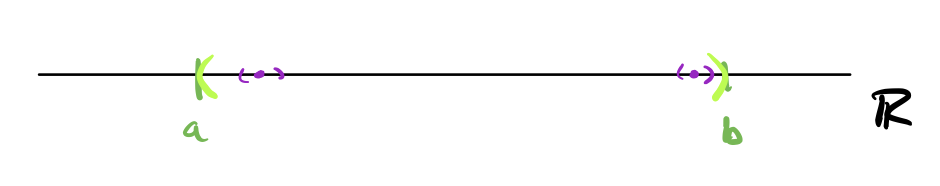
\includegraphics[scale=.75]{open_relative_r.png}
			\end{center}
		\end{figure}
		\item $(a,b)$ is \emph{not} an open subset of $\RR^2$. Indeed, any ball around a point $x \in (a,b) \subset \RR$ will leave the $x$-axis and intersect with points in the second dimension. Thus no point of $(a,b)$ is interior relative to $\RR^2$.
		\begin{figure}[H]
			\begin{center}
				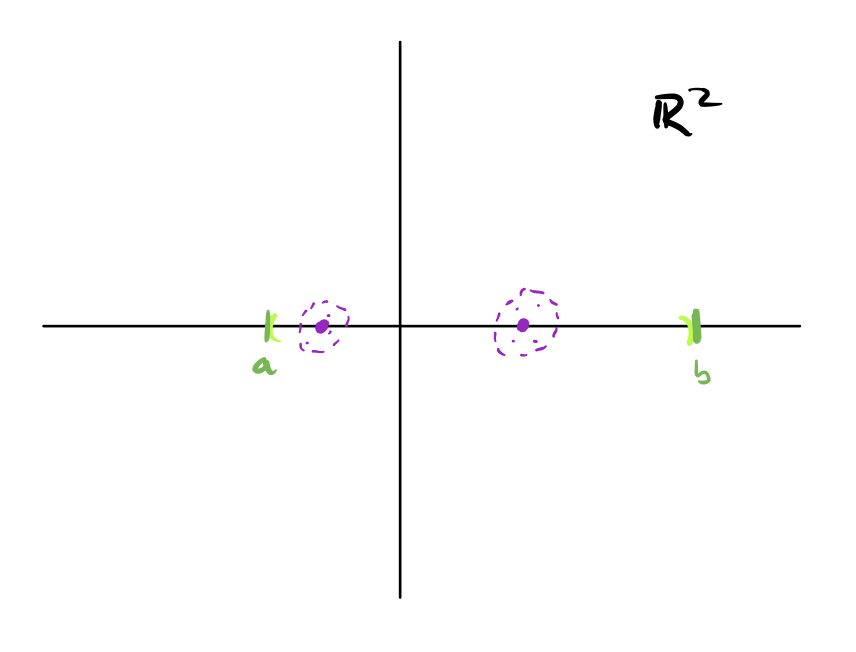
\includegraphics[scale=.75]{open_relative_r2.png}
			\end{center}
		\end{figure}  
	\end{enumerate}
\end{example}


\begin{theorem}[Relative open sets]
	Let $Y \subset X$. A subset $E$ of $Y$ is open relative to $Y$ if and only if $E = Y \cap G$ for some open subset $G$ of $X$. 
\end{theorem}
\begin{proof}
	\textcolor{red}{[[Todo]]}
\end{proof}

\begin{example}[Relative open sets]
	Let $X = \RR$ and $A = [0,1]$. Observe that $B = [0,\frac{1}{2}) \subset A \subset X$ is open in $A$, but not open in $X$. However, there exists a $C$ open in $X$ such that $B = C \cap A$. One example is $C = (-\frac{1}{2}, \frac{1}{2})$.
\end{example}	


\begin{definition}[Continuous]
	Suppose $X$ and $Y$ are metric spaces, $E \subset X$, $p \in E$, and $f$ maps $E$ into $Y$. Then $f$ is \navy{continuous} at $p$ if for every $\e > 0$ there there exists a $\d > 0$ such that for all $x \in E$ for which $d_X(x,p) < \d$, we have that $d_Y(f(x), f(p)) < \e$. 
\end{definition}

\begin{definition}[Uniformly Continuous]
	Let $f$ be a mapping of a metric space $X$ into a metric space $Y$. We say that $f$ is \navy{uniformly continuous} on $X$ if for every $\e > 0$ there exists a $\d > 0$ such that for all $p,q \in X$ for which $d_X(p,q) < \delta$, we have $d_Y(f(p),f(q)) < \e$. 
\end{definition}

\begin{definition}[Dense] TFAE: $E$ is \navy{dense} in $X$ if
\begin{enumerate}
	\item  Every point of $X$ is a limit point of $E$ or a point of $E$ (or both). 
	\item $\bar{E} = X$.
	\item $\forall \e > 0$ and $\forall x \in X$ we have that $B(x,\e) \cap E \neq \emptyset$.
\end{enumerate} 
\end{definition}

\begin{theorem}[Functions, inverses, and subsets]
	Let $f: X \to Y$
	\begin{enumerate}
		\item $E \subset Y \imp f(\inv{f}(E)) \subset E$ 
		\item $E \subset X \imp f(\inv{f}(E)) \supset E$
	\end{enumerate}
\end{theorem}



\subsection{Basic Definitions}

\begin{definition}[Open Cover]
	Let $I$ be an arbitrary index set. A collection $(G_i)_{i \in I}$ of open sets $G_i \subset X$ is called an \navy{open cover} of $X$ if $X \subset \cup_{i \in I} G_{i}$.
\end{definition}

\begin{definition}[Compact]
	$X$ is \navy{compact} if every open cover of $X$ contains a finite subcover. More explicitly, for every open cover $(G_i)_{i \in I}$ there exists $m \in \NN$ and $i_1, i_2, \ldots, i_m \in I$ such that $X \subset \cup_{j=1}^m G_{i_j}$.
	\begin{remark}
		This is also called the Heine-Borel property. 
	\end{remark}
\end{definition}

\begin{definition}[Compact subset]
	A subset $A \subset X$ is called \navy{compact subset} if $(A,d\vert_{A\times A})$ is a compact metric space. $d\vert_{A\times A}$ is the restriction of $d$ to $A \times A$.  
\end{definition}

\begin{theorem}[Heine-Borel]
	A subset $A \subset \RR^n$ is compact if and only if $A$ is closed and bounded.
\end{theorem}

\begin{definition}[Relatively compact or precompact]
	A subset $A \ss X$ is called \navy{relatively compact} or \navy{precompact} if the closure $\bar{A} \ss X$ is compact. 
\end{definition}

\begin{example}[Any finite metric space is compact]
	Let $X = \Set{x_i}_{i=1}^n$ be a finite metric space. Let $J$ be an arbitrary index set, and let $(G_j)_{j \in J}$ be an open cover of $X$. Therefore, each $x_i$ must be in at least one $G_j$. Suppose that $x_i \in G_{j_i}$, $j_i \in J$. Then $\cup_{i=1}^n G_{j_i}$ is a finite subcover. 
\end{example}

\begin{example}[$K = \Set{0} \cup \Set{1/n}_{n=1}^\infty \subset \RR$ is compact.]
	Let $J$ be an arbitrary index set, and let $(G_j)_{j \in J}$ be an open cover of $K$. First note that $0$ must be contained in some element of the open cover; call it $G_i$. Since $G_i$ is open, each element of $G_i$ is an interior element, so there exists a ball around $0$ of radius $\e > 0$ contained in $G_i$. The ball also contains all the elements of $K$ for which $n > \frac{1}{\e}$. Then, each for each of the finitely many $n \leq \frac{1}{\e}$ there exists a $G_{j_n}$ that contains $\frac{1}{n}$. Therefore every open cover has a finite subcover.
\end{example}

\begin{example}[Compactness and relative compactness in $\RR$]
	Any closed and bounded interval $[a,b]$ in $\RR$ is compact. Half open intervals $[a,b), (a,b]$ and open intervals $(a,b)$ in $\RR$ are relatively compact, since their closures are closed and bounded intervals (assuming $b$ finite). 
\end{example}

\begin{example}[Unit circle in $\RR^n$ compact]
	The set $C = \Set{x \in \RR^n; \sum_{i=1}^n \abs{x_i}^2=1} \subset \RR^n$ is compact. To show closedness, consider the map $f: \RR^n \to \RR$ defined by $f(\vx) = \sum_{i=1}^n x_i^2$, $\vx \in \RR^n$. This map is continuous (since it is the sum of continuous functions). Then $C = f^{-1}(\Set{1})$, and the singleton $\Set{1}$ is a closed set in $\RR$. To show boundedness, note that no single element of a vector can have an absolute value greater than one. Therefore $C \subset [-1,1]^n$. $C$ is closed and bounded, and by Heine-Borel, compact. 
\end{example}


\begin{example}[Orthogonal matrices]
	The set of orthogonal $n \times n$ matrices with real entries (call this $O(n,\RR)$) is compact as a subset in $\RR^2$. To see this, let $M_n$ be the set of all $n\times n$ matrices with real entries. Define a function $f: M_n \to M_n$ where $f(A) = A^T A$. This mapping is continuous. To see this, first note that $f: A \to A$ is the identity map and hence continuous. Also $f: A \to A^T$ is continuous: this follows since $\norm{A} = \norm{A^t}$, so
	\begin{align*}
		\norm{f(A) - f(B)} &= \norm{B^t - A^t} \\
		&= \norm{(B - A)^t} \\
		&= \norm{B - A} 
	\end{align*}
	Thus whenever $\norm{B - A} < \e$, we have $\norm{f(A) - f(B)} < \e$ (hence we set $\d = \e$). The product of two continuous functions is continuous.  

	Since an orthogonal matrix $O$ has inverse $O^T$, we have that $\inv{f}(I) = O(n,\RR)$. The continuity of $f$ implies that $O(n,\RR)$ is closed since it is the preimage of a singleton (which is a closed set).

	To show boundedness, recall that the columns of orthogonal matrices are orthonormal. Therefore, the absolute value of an element cannot be larger than $1$ in absolute value. Thus $O(n,\RR) \subset [-1,1]^{n^2}$. Then by Heine-Borel, $O(n,\RR)$ is compact. 
\end{example}

\begin{theorem}[Compact subsets of metric spaces are closed.]
\end{theorem}
\begin{proof}
	Let $X$ be a metric space and $K$ a compact subset of $X$. To show $K$ is closed, we will show that its complement $K^c$ is open. To do this, we must show that for all $p \in K^c$, there exists a neighborhood of $p$ completely contained in $K^c$ (and hence does \emph{not} intersect $K$). 

	Let $q \in K$. We will construct two types of neighborhoods:
	\begin{align*}
		W_q &= \Set{x \in X; d(x,q) < \frac{1}{2} d(p,q)} \tag{neighborhood of $q$} \\
		V_q &= \Set{x \in X; d(x,p) < \frac{1}{2} d(p,q)} \tag{neighborhood of $p$}
	\end{align*}
	
	Notice that the union of all $W_q$ forms an open cover of $K$. Since $K$ is compact, this open cover must have a finite subcover, $W = \bigcup_{i=1}^n W_{q_i}$. Define $V = \bigcap_{i=1}^n V_i$, which is still a neighborhood of $p$. By construction (since we have used open balls), $V_{q_i} \cap W_{q_i} = \emptyset$. Since $V \subseteq V_{q_i}$, $V \cap W_{q_i} \subseteq V_{q_i} \cap W_{q_i} = \emptyset$.  Therefore
	\begin{align*}
		V \cap W = (V \cap W_1) \cup \cdots \cup (V \cap W_n) = \emptyset
	\end{align*}
	
	Since $K \subseteq W$, we have that $V \subseteq K = \emptyset$. Thus $V$ is a neighborhood of $p$ completely contained in $K^c$. Since $p$ was arbitrary, $K^c$ is open, and $K$ is closed. 
	
	
	\begin{figure}[H]
		\begin{center}
			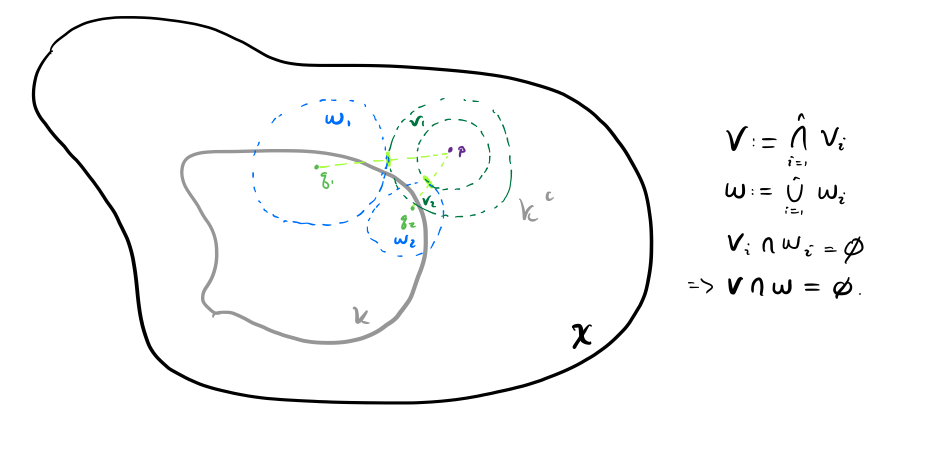
\includegraphics[scale=.45]{compact_closed.png}
		\end{center}
	\end{figure}
\end{proof}


\begin{theorem}[Closed subsets of compact sets are compact.]
\end{theorem}
\begin{proof}[Proof with compactness.]
	Let $F \subset K \subset X$, where $F$ is closed (relative to $X$) and $K$ is compact. Let $(G_\alpha)_{\alpha \in I}$ be an open cover of $F$. Since $F$ is closed, $F^c$ is open and $F^c \cup (G_\alpha)_{\alpha \in I}$ is an open cover of $K$. $K$ is compact, so every open cover has a finite subcover: $K \subset F^c \cup (G_{\alpha_i})_{i=1}^n$. Since $F \subset K$, this finite open cover also covers $F$, but clearly we don't need $F^c$ in the cover. Therefore $F$ has a finite subcover: $F \subset (G_{\alpha_i})_{i=1}^n$.

	\begin{figure}[H]
		\begin{center}
			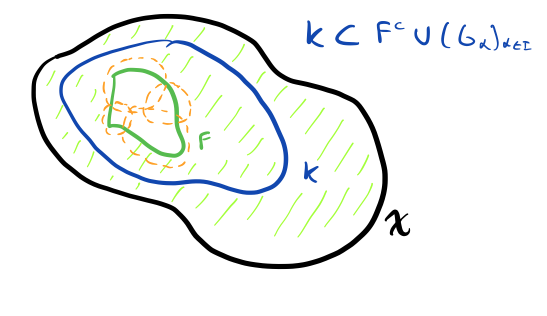
\includegraphics[scale=.45]{closed_subsets_compact.png}
		\end{center}
	\end{figure}
\end{proof}

\begin{proof}[Proof with sequential compactness.]
	Let $F \subset K \subset X$, where $F$ is closed (relative to $X$) and $K$ is compact. Let $(x_n)$ be a sequence of points in $F$ (so is also in $X$). Since $X$ is sequentially compact, there is a subsequence $(x_{n_k})$ converging to some point $x \in X$. Since $F$ is closed, $x \in X$. Therefore $F$ is sequentially compact since every sequence in $F$ has a convergent subsequence. 
\end{proof}

\begin{theorem}[The intersection of a nested sequence of compact nonempty sets is compact and nonempty.]
\end{theorem}
\begin{proof}
	Let $(A_n)$ be a sequence of compact nonempty sets. 
	\textbf{Compact:} We know that each $A_n$ is closed. The intersection of closed sets is closed, so $\cap A_n$ is closed. Notice that $\cap A_n \ss A_1$ is a closed subset of a compact set, so is also compact. 

	\textbf{Nonempty:} Since each $A_n$ is nonempty, fix an $a_n \in A_n$. The sequence $(a_n) \ss A_1$. Sequential compactness of $A_1$ implies that there is a subsequence $(a_{n_k})$ converging to some point $a \in A_1$. Notice that this limit must also be in $A_2$, since the sequence $(a_{n_k})$ is also in $A_2$ (except for potentially the first term, which does not affect convergence). This holds for all $A_n$, so $p \in \cap A_n$, which shows the intersection is nonempty.   
\end{proof}


\begin{theorem}[]
	Let $X$ be a compact metric space. Then there exists a countable, dense set $E \subset X$. 
\end{theorem}
\begin{proof}
	We will show that $\forall \e >0$ and $\forall x \in X$ we can find a a set $E$ such that for each open ball in $X$ we have that $B(x,\e) \cap E \neq \emptyset$. Fix $\e > 0$ and define an open cover of $X$ as follows:
	\begin{equation}
		B_n = \bigcup_{x \in X} B(x,\frac{1}{n})
	\end{equation}
	$X$ is compact so the open cover $B_n$ must have a finite subcover. Let $E$ be the union of the centers of the balls of each finite subcover. $E$ is the countable union of finite sets, so it is countable. Now fix $x \in X$. Choose $n$ such that $\e < \frac{1}{n}$. Since $B_n$ covers $X$, there must be some ball centered at a point of $E$, call it $y$, that contains $x$. Thus $d(x,y) < \frac{1}{n} < \e$. Thus $y \in B(x,\e) \cap E$. 
\end{proof}


\subsection{Compactness and Continuity}

\begin{theorem}[Continuous mappings on compact sets are uniformly continuous.]
	Let $X,Y$ be metric spaces and assume $X$ is compact. If $f: X \to Y$ is continuous, then it is uniformly continuous. 
\end{theorem}
\begin{proof}
	Fix $\e > 0$. \textbf{Goal:} We need to find a $\d > 0$ such that for all $x,y \in X$ for which $d_X(x,y) < \d$, we have $d_Y(f(x),f(y)) < \e$. 

	\textbf{Use continuity to create balls of points (which cover) $X$ and are mapped by the function:} Since $f$ is continuous, we know that for each $x \in X$, there exists a number $\d_x > 0$ such that for all $y \in X$ for which $d_X(x,y) < \d_x$, we have that $d_Y(f(x),f(y)) < \e/2$. Now, let $B_x$ be a ball of radius $\d_x/2$ centered at $x$. Formally, we can write
	\begin{equation*}
		B_x = B(x, \d_x / 2) = \{y \in X | d_X(x,y) < \d_x /2 \} 
	\end{equation*}
	Then $(B_x)_{x\in X}$ is an open cover of $X$. 

	\textbf{Use compactness to select a finite subcover of these balls and use the smallest radius to create uniformity:} By compactness, there exists a finite subcover of $X$. Let $x_1, \ldots, x_m$ be the $x$ which generate this finite subcover. Define $\d > 0$ as follows
	\begin{equation}
		\d = \frac{1}{2} \min (\d_{x_1}, \ldots, \d_{x_m})
	\end{equation}
	(notice that $\d$ is indeed positive, since we are taking the minimum of finitely many positive numbers).

	\textbf{Show that our choice of $\d$ works:} Fix $x,y \in X$ such that $d_X(x,y) < \d$. There exists and index $i \in \{1, \ldots, m\}$ such that $x \in B_{x_i}$ (i.e., an element of $X$ is in some ball of the finite subcover). Then
	\begin{equation}
		d_X(x_i,y) \leq d_X(x_i, x) + d_X(x,y) < \frac{1}{2} \d_{x_i} + \d < \d_{x_i} 
	\end{equation} 
	Now, using the definition of $\d_{x_i}$, we have that
	\begin{equation}
		d_Y(f(x),f(y)) \leq d_Y(f(x),f(x_i)) + d_Y(f(x_i),f(y)) \leq \e/2 + \e/2 = \e
	\end{equation}
	since $d_X(x_i, x) < \d_x / 2 < \delta_x$ so continuity implies $d_Y(f(x),f(x_i)) < \e / 2$, and  $d_X(x_i,y) < \d_{x_i}$ so continuity implies  $d_Y(f(x_i),f(y)) < \e /2$.
\end{proof}

\begin{theorem}[The image of a continuous function which maps from a compact set is compact]
	Let $X,Y$ be metric spaces and assume $X$ is compact. If $f: X \to Y$ is continuous, then $f(X) \subset Y$ is compact. 
\end{theorem}
\begin{proof}[Proof with compactness]
	Let $(V_i)_{i \in I}$ be an open cover of $f(X)$. Since $f$ is continuous, we have that $U_i = f^{-1}(V_i) \subset X$ is open for each $i$. Note that $U \ss \inv{f}(f(U))$ for every $U \subset X$. Therefore
	\begin{equation}
		X \ss \inv{f}(f(X)) \ss \cup_{i \in I} \inv{f}(V_{i}) = \cup_{i \in I} U_{i} 
	\end{equation}
	which shows that $\cup_{i \in I} U_{i}$ is an open cover of $X$ (the second subset relation uses that applying $f^{-1}$ preserves unions). Since $X$ is compact, there are finitely many indices, say up to $m$, such
	\begin{equation}
		X \ss \bigcup_{j=1}^m  U_{i_j}
	\end{equation}
	Applying $f$ preserves inclusions and $V \supset f(\inv{f}(V))$, so we have that
	\begin{equation}
		f(X) \ss \bigcup_{j=1}^m f(U_{i_j}) \ss \bigcup_{j=1}^m V_{i_j}
	\end{equation}
	Thus every open cover of $f(X)$ has a finite subcover, so $f(X)$ is compact. 
\end{proof}

\begin{proof}[Proof with sequential compactness]
	Let $(y_n)$ be a sequence in $f(X) \ss Y$. For each $n \in \NN$ choose a point $x_n$ such that $f(x_n) = y_n$. By sequential compactness of $X$, there is some subsequence $(x_{n_k})$ converging to a point $x \in X$. The continuity of $f$ implies that $f(x_{n_k})$ converges to $f(p) \in f(X)$. Therefore every sequence in $f(X)$ has a convergent subsequence, so $f(X)$ is sequentially compact.  
\end{proof}


\begin{theorem}[Functions from compact sets to the reals achieve their minimum and maximum values]
	Let $X$ be a compact metric space and $f:X \to \RR$ a continuous function. Then there exists $x_0 \in X$ such that $f(x_0) = \sup_{x\in X} f(x)$. 
\end{theorem}
\begin{proof}
	Since $X$ is compact, we know that the image $f(X)$ is also compact. Since $f(X) \ss \RR$, the Heine-Borel theorem tells us that $f(X)$ is closed and bounded. Completeness of the real numbers (every nonempty subset of the real numbers that is bounded above has a supremum in $\RR$). Since $f(X)$ is closed, this supremum must be contained in $f(X)$. Therefore there exists $x_0 \in X$ such that $f(x_0) = \sup_{x\in X} f(x)$. 
\end{proof}



\subsection{Sequential Compactness and Total Boundedness}

\begin{definition}[Sequentially compact]
	A metric space $X$ is \navy{sequentially compact} if every sequence in $X$ has a convergent subsequence. 
	\begin{remark}
	This is also called the Bolzano-Weierstrass property. Recall that the Bolzano-Weierstrass theorem states that every bounded sequence in $\RR^n$ has a convergent subsequence. 
	\end{remark}	
\end{definition}

\begin{example}[Finite sets are sequentially compact]
	Suppose $(x_n)$ is a sequence contained in a finite set. Then this sequence must repeat a term infinitely often. Define the subsequence which is constant at this term: this subsequence clearly converges. 
\end{example}

\begin{theorem}[(Sequentially) compact sets are closed and bounded]
\end{theorem}
\begin{proof}
	Let $A$ be a sequentially compact subset of a metric space $X$.

	\textbf{Closed:} Let $p$ be a limit point of $A$. Then there is a sequence $(a_n)$ in $A$ that converges to $p$. Sequential compactness of $A$ implies that there is a subsequence of $(a_{n_k})$ which converges to some $q \in A$. However every subsequence of a convergent sequence must converge to the same limit as the full sequence, which implies $p=q \in A$. Therefore $A$ is closed. 

	\textbf{Bounded:} Fix a point $x \in X$. Suppose $A$ is not bounded. Then for each $n \in \NN$ there must be some point $a_n$ such that $d(x,a_n) \geq n$. However, sequential compactness implies that some subsequence $(a_{n_k})$ must converge. Convergent sequences are bounded, so we cannot have that $d(x,a_{n_k}) \to \infty$ as $k \to \infty$. Thus the sequence $(a_n)$ cannot behave as assumed, and it must be that $A$ is bounded for some $r \in \RR$. 

\end{proof}


\begin{definition}[Bounded metric space]
	A metric space $X$ is \navy{bounded} if it fits in a single fixed ball. More precisely, there exists some $x_0 \in X$ and $r > 0$ such that $X \subseteq B(x_0,r)$. 
\end{definition}

\begin{definition}[Totally bounded]
	A metric space $X$ is \navy{totally bounded} if for every $\e > 0$ there exist finitely many balls of radius $\e$ that cover $X$. 
\end{definition}

\begin{claim}[Totally bounded implies bounded]
	Let $X$ be a totally bounded metric space. Then it is bounded. 
\end{claim}
\begin{proof}
	Fix $\e > 0$ and $x,y \in X$. Total boundedness implies there exists points $(x_i)_{i=1}^n$ such that $X \subseteq \bigcup_{i=1}^n B(x_i, \e)$. Suppose $x \in B(x_i,\e)$ and $y \in B(x_j,\e)$. Then 
	\begin{equation}
	 	d(x,y) \leq d(x,x_i) + d(x_i, x_j) + d(x_j,y) < d(x_i, x_j) + 2\e
	 \end{equation} 
	 There are only finitely many values of $d(x_i, x_j)$ we can set $M = \max_{i,j} d(x_i, x_j)$. Therefore $d(x,y) < M + 2\e$. Therefore $X$ is bounded. 
\end{proof}


\begin{example}[Closed and bounded interval in $\RR$ is totally bounded]
	A closed and bounded interval $I = [a,b] \subset \RR$ is totally bounded. 
\end{example}

\begin{example}[Bounded but not totally bounded]
	The following are examples of metric spaces which are bounded but not totally bounded.
	\begin{enumerate}
		\item $\ell^1$-space is defined to be the collection of all sequences $(a_n)_n$ with $\sum_{n=1}^\infty |a_n| < \infty$. We define a distance $d$ on $\ell^1$ as follows: $d\parens{(a_n)_n, (b_n)_n} = \sum_{n=1}^\infty |a_n - b_n|$. The unit ball of $\ell^1$ centered at the zero-element (call this call $B_1$) (i.e., the zero sequence) is bounded but not totally bounded. More precisely, 
		\begin{equation}
			B_1 = \Set{(a_n)_n; \sum_{n=1}^\infty |a_n| \leq 1}
		\end{equation}
		Boundedness is clear. Consider the the set of sequences $A = \Set{a_n}$ where each $a_n$ is zero except for a 1 in the $n$-th entry. Each $a_n \in B_1$. However, 
		\begin{equation}
			d(a_n,a_m) = 
			\begin{cases}
				2 & n \neq m \\
				0 & n = m
			\end{cases} 	
		\end{equation} 
		If we take balls of radius $\e = \frac{1}{2}$, then a ball can cover at most one sequence in $A$. Therefore we can't cover $A$ with finitely $\e$-balls and hence can't cover $B_1$ with finitely many $\e$-balls, so that $B_1$ is not totally bounded. 
		\item $\ell^\infty$-space is defined to be the collection of all sequences $(a_n)_n$ with $\sup_n |a_n| < \infty$. We define a distance $d$ on $\ell^\infty$ as follows: $d\parens{(a_n)_n, (b_n)_n} = \sup_n \abs{a_n - b_n}$. Using the same set of sequences as the previous example, note that for all $n$ we have that
		\begin{equation}
		   	d\parens{a_n, \Set{0}_{n=1}^\infty} = 1
		\end{equation}   
		so that $A \ss B_1$ (with the sup norm). Further,
		\begin{equation}
			d(a_n,a_m) = 
			\begin{cases}
				1 & n \neq m \\
				0 & n = m
			\end{cases} 	
		\end{equation}
		But again, if we take balls of radius $\e = \frac{1}{2}$, then a ball can cover at most one sequence in $A$. Therefore we can't cover $A$ with finitely $\e$-balls and hence can't cover $B_1$ with finitely many $\e$-balls, so that $B_1$ is not totally bounded. 
	\end{enumerate}
\end{example}


\begin{theorem}[Characterizations of compactness]
	Let $X$ be a metric space. The following are equivalent:
	\begin{enumerate}
		\item $X$ is compact.
		\item $X$ is sequentially compact.
		\item $X$ is totally bounded and complete. 
	\end{enumerate}
\end{theorem}

\begin{proof}[Proof of $X$ is compact $\imp$ $X$ is sequentially compact]
	We argue by contradiction. Suppose $X$ is compact but not sequentially compact. Thus there must exist some sequence $(x_n)_n \ss X$ without a convergence subsequence. Let $A$ be the range of the sequence (more explicitly, $A = \Set{x_n; n \in \NN}$). Note that $A$ has to be an infinite (if $A$ were finite, then there would be a constant subsequence, which is convergent). 

	Further, $A$ cannot have any limit points (by definition, a point is a limit point of a sequence if there exists a subsequence converging to it). Therefore for each $x_n$, we can find an open ball centered at $x_n$ that only intersects $A$ at $x_n$: $B_n \cap A = \Set{x_n}$. $A$ is also closed (since it has no limit points), so that $X-A$ is open. We can construct an open cover of $X$ as:
	\begin{equation}
		X \subseteq \bigcup_{n} B_n \cup \Set{X-A}
	\end{equation}
	Compactness of $A$ implies this open cover has a finite subcover. Therefore the finite subcover can only contain finitely many of the sets in $\bigcup_{n} B_n$, so can only contain finitely many of the points in $A$, which is a contradiction to the covering. 
\end{proof}

\begin{proof}[Proof of $X$ is sequentially compact $\imp$ $X$ is totally bounded and complete]
	Suppose $X$ is sequentially compact. 

	\textbf{Complete}: Fix $\e > 0$. Let $(x_n)_n \ss X$ be a Cauchy sequence. Sequential compactness implies $(x_n)_n$ has a convergent subsequence. Call this subsequence $(x_{n_k})$ and its limit $x$. Then there exists an $N$ such that $d(x_{n_k},x) < \e$ for all $n_k \geq N$. Since $(x_n)_n$ is Cauchy, there exists an $N$ such that $n,m \geq M$ implies that $d(x_n,x_m) < \e$. But then
	\begin{equation}
		d(x_n,x) \leq d(x_n, x_{n_k}) + d(x_{n_k}, x) < 2\e
	\end{equation}
	for all $n, n_k \geq \max\{N,M\}$. Therefore $(x_n)_n$ converges, so $X$ is complete. \textbf{In words, Cauchy sequences with convergence subsequences also converge.} 

	\textbf{Totally Bounded:} We argue by contradiction. Suppose $X$ is not totally bounded. Then there exists an $\e > 0$ such that $X$ cannot be covered by finitely many balls of radius $\e$. We know that 1 ball of radius $\e$ cannot cover $X$. Therefore there must be a point of $X$ outside of this ball: call it $x_1$. Similarly, 2 balls of radius $\e$ cannot cover $X$, so pick a point outside of these two balls and call it $x_2$. Proceeding in this manner generates an infinite sequence. Now consider the $n$-th term of this sequence. When we choose $n+1$, we must be able to choose a point such that $d(x_i, x_{n+1}) \geq \e$ for all $i \in \intsfin{n}$. Otherwise, we would have that $X \subseteq \bigcup_{i=1}^n B(x_i,\e)$, which would be a contradiction to $X$ not being totally bounded. Thus we can construct such a sequence. 

	Next, since $X$ is sequentially compact, we must be able to find a convergence subsequence. However, the sequence we've constructed has $d(x_i, x_j) \geq \e$ for all $i,j \in \NN$ (hence no subsequence can be Cauchy, and we know that convergence sequences are Cauchy). Therefore we have reached a contradiction and it holds that $X$ is totally bounded. 
\end{proof}

\begin{proof}[Proof of $X$ is totally bounded and complete $\imp$ $X$ is sequentially compact]
	Suppose $X$ is totally bounded and complete. Let $(x_n)_n \ss X$ be a sequence. \textbf{We will construct an convergent subsequence.} By the definition of total boundedness, for all $\e > 0$, $X$ can be covered by finitely many balls of radius $\e$. \textbf{Observation:} One of these balls must contain infinitely many points of $(x_n)_n$. This inspires the following process: 
	\begin{enumerate}
		\item \textbf{Step 1:} Cover $X$ with balls of radius 1. One of these balls must contain infinitely many points of $(x_n)_n$. These infinitely many points form a subsequence, call it $(x^{(0)}_n)_n$. 
		\item \textbf{Step 2:} Cover $X$ with balls of radius $\frac{1}{2}$. One of these balls must contain infinitely many points of $(x^{(0)}_n)_n$. These infinitely many points form a subsequence, call it $(x^{(1)}_n)_n$. 
		\item \textbf{Step $\bm n$:} Cover $X$ with balls of radius $\frac{1}{2^n}$. One of these balls must contain infinitely many points of $(x^{(n-1)}_n)_n$. These infinitely many points form a subsequence, call it $(x^{(n)}_n)_n$.
	\end{enumerate}
	Therefore we have founded nested sequences: $(x^{(0)}_n)_n \ss (x^{(1)}_n)_n \ss \cdots \ss (x^{(n-1)}_n)_n \cdots$. Set $a_n = x^{(n)}_n$ (which is a subsequence of $(x_n)_n$). 

	\textbf{Now we show that $a_n$ is a Cauchy sequence.} Fix $\e > 0$ and choose $N$ such that $2^{-N + 1} < \e$. Now for $m > n \geq N$ we have that
	\begin{equation}
		d(a_m, a_n) < 2 \cdot 2^{-n} < 2^{-N + 1} < \e
	\end{equation}
	since $a_m$ and $a_n$ are contained in the same ball of radius $2^{-n}$. Therefore $(a_n)_n$ is a Cauchy sequence, and completeness implies it converges. 

	\textbf{We have found a convergence subsequence, so $X$ is sequentially compact.} 

	\begin{figure}[H]
		\begin{center}
			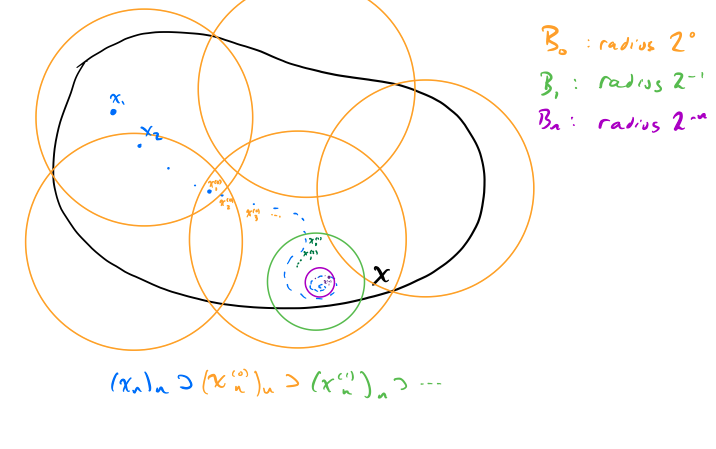
\includegraphics[scale=.55]{totally_bounded_complete_compact.png}
		\end{center}
	\end{figure}

\end{proof}

\subsection{Equicontinuity and the Arzela-Ascoli Theorem}

[[To prove relatively compact, we construct a sequence of functions that converges uniformly.]]

\newpage

\section{Approximation Theory and Fourier Series}

\subsection{Orthonormal Systems}

\begin{theorem}[Best $L^2$-approximation]
	Let
	\begin{itemize}
		\item $(\phi_n)_n$ be an orthonormal system 
		\item $f \in pc([a,b])$
		\item $c_n = \angles{f,\phi_n}$
	\end{itemize}
	Define
	\begin{itemize}
		\item $s_N(x) = \sum_{n=1}^N c_n \phi_n(x)$
		\item $t_N(x) = \sum_{n=1}^N b_n \phi_n(x)$ for arbitrary coefficients $b_1,\ldots,b_N \in \CC$
	\end{itemize}
	Then
	\begin{equation}
		\norm{f - s_N}_2 \leq \norm{f - t_N}_2
	\end{equation}
	and equality holds iff $b_n = c_n$ for all $n=1,\ldots,N$.
\end{theorem}

\begin{proof}
We compute the following elements:
\begin{align*}
	\angles{f,t_N} = \sum_{n=1}^N \overline{b}_n \angles{f,\phi_n} = \sum_{n=1}^N \overline{b}_n c_n
\end{align*}

\begin{align*}
	\angles{f,s_N} = \sum_{n=1}^N \overline{c}_n \angles{f,\phi_n} = \sum_{n=1}^N \overline{c}_n c_n = \sum_{n=1}^N \abs{c_n}^2
\end{align*}


\begin{align*}
	\angles{t_N,t_N} &= \angles{\sum_{n=1}^N b_n\phi_n, \sum_{m=1}^N b_m \phi_m} \\
	&= \sum_{n=1}^N \sum_{m=1}^N b_n \overline{b}_m \angles{\phi_n, \phi_m} \\
	&= \sum_{n=1}^N \abs{b_n}^2 \tag{$(\phi_n)_n$ orthonormal}
\end{align*}

Then
\begin{align*}
	\norm{f-t_N}^2_2 &= \angles{f-t_N,f-t_N} \\
	&= \angles{f,f} - \angles{f,t_N} - \angles{t_N,f} + \angles{t_N,t_N} \\
	&= \angles{f,f} - \sum_{n=1}^N \overline{b}_n c_n - \sum_{n=1}^N b_n \overline{c}_n + \sum_{n=1}^N \abs{b_n}^2 \\
\end{align*}

\begin{align*}
	\abs{b_n - c_n}^2 &= (b_n - c_n)(\overline{b_n - c_n}) \\
	&= (b_n - c_n)(\overline{b_n} - \overline{c_n}) \\
	&= b_n \overline{b_n} - b_n \overline{c_n} - c_n \overline{b_n} + c_n \overline{c_n} \\
	&= \abs{b_n}^2 - b_n \overline{c_n} - c_n \overline{b_n} + \abs{c_n}^2
\end{align*}

Therefore
\begin{align*}
	\norm{f-t_N}^2_2 &= \angles{f,f} - \sum_{n=1}^N \overline{b}_n c_n - \sum_{n=1}^N b_n \overline{c}_n + \sum_{n=1}^N \abs{b_n}^2 \\
	&= \angles{f,f} + \sum_{n=1}^N \abs{b_n - c_n}^2 - \sum_{n=1}^N \abs{c_n}^2 
\end{align*}

And
\begin{align*}
	\norm{f-s_N}^2_2 &= \angles{f-s_N,f-s_N} \\
	&= \angles{f,f} - \angles{f,s_N} - \angles{s_N,f} + \angles{s_N,s_N} \\
	&= \angles{f,f} - 2 \sum_{n=1}^N \abs{c_n}^2 + \sum_{n=1}^N \abs{c_n}^2 \\
	&= \angles{f,f} - \sum_{n=1}^N \abs{c_n}^2
\end{align*}

Finally
\begin{align*}
	\norm{f-t_N}^2_2 = \norm{f-s_N}^2_2 + \sum_{n=1}^N \abs{b_n - c_n}^2
\end{align*}
Thus the claim follows. Indeed, for equality to be achieved, we must have that $b_n = c_n$ for $n=1,\ldots,N$. 

\end{proof}

\begin{theorem}[Bessel's Inequality]
	If $(\phi_n)_n$ is an orthonormal system on $[a,b]$ and $f \in pc([a,b])$, then
	\begin{equation}
		\sum_{n} \abs{\angles{f,\phi_n}}^2 \leq \norm{f}^2_2
	\end{equation}
\end{theorem}

\begin{proof}
	In the proof of the previous theorem, we calculated that
	\begin{equation}
		0 \leq \norm{f-s_N}^2_2 = \angles{f,f} - \sum_{n=1}^N \abs{c_n}^2
	\end{equation}
	Therefore the following holds for all $N$
	\begin{equation}
		\sum_{n=1}^N \abs{c_n}^2 \leq \angles{f,f}
	\end{equation}
	Take the limit $N \to \infty$ to get the claim
	\begin{equation}
		\sum_{n} \abs{c_n}^2 = \sum_{n} \abs{\angles{f,\phi_n}}^2 \leq \norm{f}^2_2
	\end{equation}
	(Notice that the sum $\sum_{n=1}^N \abs{c_n}^2$ converges.)
\end{proof}

\begin{corollary}[Riemann-Lebesgue Lemma]
	Let $(\phi_n)_n$ be an orthonormal system and $f \in pc([a,b])$, then
	\begin{equation}
		\lim_{n\to\infty} \angles{f,\phi_n} = 0
	\end{equation}
\end{corollary}

\begin{proof}
	In the proof of Bessel's inequality, we showed that the series $\sum_{n} \abs{\angles{f,\phi_n}}^2$ converges. Therefore, a necessary condition of convergence, is that the terms go to zero. 
\end{proof}


\begin{definition}[Complete Orthonormal System]
	An orthonormal system $(\phi_n)_n$ is called \navy{complete} if 
	\begin{equation}
		\sum_{n=1}^\infty \abs{\angles{f,\phi_n}}^2 = \norm{f}^2_2 \quad \forall f \in pc([a,b])
	\end{equation}
\end{definition}

\begin{theorem}[]
	Let
	\begin{itemize}
		\item $(\phi_n)_n$ be an orthonormal system 
		\item $s_N(x) = \sum_{n=1}^N c_n \phi_n(x)$
	\end{itemize}
	Then $(\phi_n)_n$ is complete if and only if $(s_N)_N$ converges to $f$ in the $L^2$-norm. 

	Precisely, $\lim_{N \to \infty} \norm{f - s_N}_2 = 0$ for every $f \in \text{pc}([a,b])$). 
\end{theorem}

\begin{proof}
	Again, from the best approximation theorem, we calculated that
	\begin{equation}
		\norm{f - s_N}^2_2 = \angles{f,f} - \sum_{n} \abs{\angles{f,\phi_n}}^2 
	\end{equation}
	Then this converges to $0$ if and only if $(\phi_n)_n$ is complete.
\end{proof}



\subsection{Trigonometric Polynomials}

\begin{definition}[Trigonometric Polynomial, Degree]
	A \navy{trigonometric polynomial} is a function of the form
	\begin{equation}
		f(x) = \sum_{n=-N}^N c_n e^{2\pi i n x} \quad x \in \RR
	\end{equation}
	where $N \in \NN$ and $c_n \in \CC$. The largest $N$ for which either $c_N$ or $c_{-N}$ is non-zero is called the \navy{degree} of $f$. 
\end{definition}


\begin{claim}[Alternative form of trigonometric polynomial]
	Every trigonometric polynomial can also be written in the form
	\begin{equation}
		f(x) = a_0 + \sum_{n=1}^N a_n \cos(2\pi n x) + b_n \sin(2\pi nx)
	\end{equation}
	for coefficients $a_n, b_n$. 
\end{claim}
\begin{proof}
	Using Euler's identity, recall that
	\begin{equation}
		e^{2\pi i n x} = \cos(2\pi i n x) + i \sin(2\pi i n x)
	\end{equation}
	Then, for $x \in \RR$,
	\begin{align*}
		f(x) &= \sum_{n=-N}^N c_n e^{2\pi i n x} \\
		&= \sum_{n=-N}^N \squares{\cos(2\pi i n x) + i \sin(2\pi i n x)} \\
		&= c_0 + \sum_{n=1}^N \squares{c_n(\cos(2\pi i n x) + i \sin(2\pi i n x)) + c_{-n}(\cos(2\pi i (-n) x) + i \sin(2\pi i (-n x))} \\
		&= c_0 + \sum_{n=1}^N \squares{(c_n + c_{-n})\cos(2\pi i n x) + i(c_n - c_{-n})\sin(2\pi i n x)}
	\end{align*}
	Therefore the claim alternative holds for ($1 \leq n \leq N$)
	\begin{align*}
		a_0 &= c_0 \\
		a_n &= c_n + c_{-n} \\
		b_n &= i(c_n - c_{-n})
	\end{align*}
	
\end{proof}

\begin{definition}[Partial sums]
	For a 1-periodic function $f \in \text{pc}$ we define the \navy{partial sums} 
	\begin{equation}
		S_Nf(x) = \sum_{n=-N}^N \hat{f}(n) e^{2\pi i nx}
	\end{equation}
\end{definition}

\begin{definition}[Convolution]
	For two 1-periodic functions $f,g \in \text{pc}$ we define their \navy{convolution} by
	\begin{equation}
		f * g(x) = \int_0^1 f(t)g(x-t)dt
	\end{equation}
\end{definition}


\begin{definition}[Approximation of Unity]
	A sequence of 1-periodic continuous functions $(k_n)_n$ is called \navy{approximation of unity} if for all 1-periodic continuous functions $f$ we have that $f * k_n$ converges uniformly to $f$ on $\RR$. That is
	\begin{equation}
		\sup_{x \in \RR} \abs{f * k_n(x) - f(x)} \to 0
	\end{equation}
	as $n \to \infty$
\end{definition}

\begin{theorem}[Sufficient conditions for approximation of unity]
	Let $(k_n)_n$ be a sequence of 1-periodic continuous functions such that
	\begin{enumerate}
		\item Non-negative: $k_n(x) \geq 0$.
		\item Integrates to 1: $\int_{-1/2}^{1/2} k_n(t) dt = 1$.
		\item ``Mass'' of $k_n$ concentrated near the origin: For all $1/2 \geq \d > 0$ we have
		\begin{equation}
			\int_{-\d}^\d k_n(t) dt \to 1 \text{ as } n \to \infty
		\end{equation}
	\end{enumerate}
\end{theorem}
\begin{proof}
	Let $f$ be a function that is 1-periodic and continuous. \textbf{What can we say about $f$?} \textbf{Using continuity:} Consider the interval $[-1/2,1/2]$. $f$ is continuous on this compact set so that  on $[-1/2,1/2]$ it is
	\begin{enumerate}
		\item Bounded
		\item Uniformly continuous
	\end{enumerate}
	\textbf{Using periodicity:} by periodicity, on all of $\RR$, $f$ is 
	\begin{enumerate}
		\item Bounded
		\item Uniformly continuous
	\end{enumerate}
	Thus there exists a $\d > 0$ such that
	\begin{equation}
		\abs{f(x-t)-f(x)} \leq \e/2 \text{ for all } |t| < \d, x \in \RR
	\end{equation}
	Then we can write 
	\begin{equation}
		f * k_n(x) - f(x) = \int_{-1/2}^{1/2} \parens{f(x-t) - f(x)} k_n(t) dt 
	\end{equation}
	Let's break this integral up into two pieces:
	\begin{align*}
		A &= \int_{|t| \leq \d } \parens{f(x-t) - f(x)} k_n(t) dt \\
		B &= \int_{1/2 \geq \d > 0} \parens{f(x-t) - f(x)} k_n(t) dt \\
	\end{align*}
	To bound $A$, we use uniform continuity and (ii):
	\begin{align*}
		|A| &= \abs{\int_{|t| \leq \d } \parens{f(x-t) - f(x)} k_n(t) dt}
	\end{align*}
	
	\improvement[inline]{Incomplete.}
\end{proof} 

\begin{theorem}[Fej\'er]
	For every 1-periodic, continuous function $f$ we have
	\begin{equation}
		\sigma_N f \to f \text{ as } N \to \infty
	\end{equation}
	uniformly on $\RR$. 

	In words, the sequence $\sigma_n$ of Ces\'aro means of the sequence $(s_n)$ of partial sums of the Fourier series of $f$ converges uniformly to $f$ on $[0,1]$.
\end{theorem}

\begin{corollary}
	Every 1-periodic continuous function can be uniformly approximated by trigonometric polynomials. 
\end{corollary}
\begin{proof}
	
\end{proof}



\begin{corollary}[Fej\'er kernel an approximation of unity]

\end{corollary}
\begin{proof}
	We must verify the hypotheses of the above theorem. 

	\improvement[inline]{Incomplete.}
\end{proof}

\begin{theorem}[Partial sum convoluted with 1-periodic, continuous function converges in 2-norm]
	Let $f$ be a 1-periodic and continuous function. Then
	\begin{equation}
		\lim_{N \to \infty} \norm{S_N f - f}_2 = 0
	\end{equation}
\end{theorem}
\begin{proof}
	Let $\e > 0$. By Fejer's theorem, there exists a trigonometric polynomial $p$ that uniformly approximates $f$: That is, $|f(x) - p(x)| < \e/2$. Then
	\begin{equation}
		\norm{f - p}_2 = \parens{\int_0^1 \abs{f(x)-p(x)}^2}^{1/2} \leq \e/2
	\end{equation}
	Suppose $p$ has degree $N$. Then 
	\begin{equation}
		S_N f - f = S_N f - S_N p + S_N p - f = S_N (f - p) + p - f
	\end{equation}
	Then by Minkowski's inequality
	\begin{equation}
		\norm{S_N f - f}_2 \leq \norm{S_N (f - p)}_2 + \norm{p - f}_2
	\end{equation}
	Bessel's inequality implies that $\norm{S_N f}_2 \leq \norm{f}_2$. Therefore $\norm{S_N (f-p)}_2 \leq \norm{f-p}_2 = \norm{p-f}_2$. Then
	\begin{equation}
		\norm{S_N f - f}_2 \leq 2 \norm{f-p}_2 \leq \e
	\end{equation}
	which proves the claim. 	
\end{proof}

\begin{corollary}[Parseval's Theorem]
	If $f,g$ are 1-periodic, continuous functions, then
	\begin{equation}
		\angles{f,g} = \sum_{n=-\infty}^\infty \hat{f}(n) \overline{\hat{g}(n)}
	\end{equation}
	As a special case
	\begin{equation}
		\norm{f}^2_2 = \sum_{n=-\infty}^\infty \abs{\hat{f}(n)}^2
	\end{equation}
\end{corollary}

\begin{proof}
	We compute
	\begin{align*}
		\angles{S_N f, g} &= \angles{\sum_{n=-N}^N \hat{f}(n) e^{2\pi i n x}, g} \\
		&= \sum_{n=-N}^N \angles{\hat{f}(n) e^{2\pi i n x}, g} \\
		&= \sum_{n=-N}^N \hat{f}(n) \angles{e^{2\pi i n x}, g} \\
		&= \sum_{n=-N}^N \hat{f}(n) \int_0^1 e^{2\pi i n x} \overline{g(x)} dx \\
		&= \sum_{n=-N}^N \hat{f}(n) \overline{\hat{g}(n)}
	\end{align*}
	Now notice that
	\begin{equation}
		\angles{S_N f, g} \to \angles{f,g}
	\end{equation}
	because
	\begin{align*}
		\abs{\angles{S_N f, g} - \angles{f,g}} &= \abs{\angles{S_N f - f, g}} \\
		&\leq \norm{S_N f - f}_2 \norm{g}_2 \tag{Cauchy-Schwarz} \\
		&\to 0 \text{ as } N \to \infty \tag{previous theorem} 
	\end{align*}
	The special case follows from setting $f=g$. 
\end{proof}


\begin{theorem}[]
	Let $f$ be a 1-periodic continuous function and let $x \in \RR$. Suppose $f$ is differentiable at $x$. Then 
	\begin{equation}
		S_N f(x) \to f(x) \text{ as } N \to \infty
	\end{equation}
\end{theorem}
\begin{proof}
	First by definition
	\improvement[inline]{Proof incomplete.}
\end{proof}



\subsection{Weierstrass Theorem}

\begin{theorem}[Weierstrass Theorem]
	For every $f \in C([a,b])$ there exists a sequence of polynomials that converges uniformly to $f$. 
\end{theorem}
\begin{proof}
	Let $\e > 0$. 

	\improvement[inline]{Incomplete.}
\end{proof}


\begin{remark}
	This shows that polynomials are dense in $C([a,b])$. 
\end{remark}


\subsection{Stone-Weierstrass Theorem}

\begin{theorem}[Stone-Weierstrass Theorem (Sufficient conditions for a subset of $C(K)$, $K$ compact, to be dense)]\label{thm:stone-weierstrass}
	Suppose 
	\begin{itemize}
		\item $K$ is a compact metric space.
		\item $\aA \ss C(K)$ such that
		\begin{enumerate}
			\item $\aA$ is a self-adjoint algebra: for $f,g \in \aA$, $c \in \CC$, we have
			\begin{equation}
				f+g \in \aA, f \cdot g \in \aA, c \cdot f \in \aA, \bar{f} \in \aA
			\end{equation}
			\item $\aA$ separates points: for all $x,y \in K$ with $x \neq y$, there exists $f \in \aA$ such that $f(x) \neq f(y)$. 
			\item $\aA$ vanishes nowhere: for all $x \in K$, there exists $f \in \aA$ such that $f(x) \neq 0$. 
		\end{enumerate}
	\end{itemize}
	\textbf{Then} $\aA$ is dense in $C(K)$ (that is, $\bar{\aA} = C(K)$). 
\end{theorem}

\begin{remark}
	Polynomials and trigonometric polynomials satisfy the conditions of the Stone-Weierstrass Theorem (Theorem \ref{thm:stone-weierstrass}).

	\improvement[inline]{Show this.}
\end{remark}

We prove a sequence of lemmas before proving the theorem. 

\begin{lemma}[Sequence of polynomial (zero intercept) uniformly converging to absolute value function]
	For every $a > 0$ there exists a sequence of polynomials $(p_n)_n$ with real coefficients such that $p_n(0) = 0$ $\forall n$ and
	\begin{equation}
		\sup_{x \in [-a,a]}\abs{p_n(x) - \abs{x}} \to 0 \text{ as } n \to \infty
	\end{equation}
\end{lemma}
\begin{proof}
	$f(x) = \abs{x}$ is a continuous function on $[-a,a]$. By Weierstrass' theorem, there exists a sequence of polynomials $(q_n)_n$ converging uniformly to $f(x) = \abs{x}$ on $[-a,a]$. Now set $p_n(x) = q_n(x) - q_n(0)$. It is clear that $p_n(0) = 0$. Further, $p_n(x)$ converges uniformly to $|x|$, since $q_n(x)$ uniformly converges to $|x|$ and $q_n(0)$ converges to 0. 

	More formally: fix $\e > 0$. Then $\exists N$ such that $|q_n(x) - |x|| < \e$ for all $n>N$ and $x \in [-a,a]$. Thus, for this $N$, $|q_n(0)|< \frac{\e}{2}$ and $|q_n(x)| < \frac{\e}{2}$ for all $x \neq 0$. Therefore
	\begin{equation}
		|p_n(x)| = |q_n(x) - q_n(0)| \leq |q_n(x)| + |q_n(0)| < \frac{\e}{2} + \frac{\e}{2} = \e
	\end{equation}
\end{proof}

\begin{lemma}[]
	If $f \in \bar{A}$, then $|f| \in \bar{A}$.
\end{lemma}
\begin{proof}
	By the previous lemma, there exists a sequence of polynomials (with zero intercept) converging uniformly to the absolute value function. Thus fix $\e > 0$. Let $a = \max_{x \in K} |f(x)|$. Then there exist coefficients $c_1,c_2,\ldots,c_N \in \RR$ such that
	\begin{equation}\label{eq:stone-weierstrassuni}
		\abs{\sum_{i=1}^n c_i y^i - \abs{y}} \leq \e \quad \forall \abs{y} \leq a
	\end{equation}
	\textbf{Note}: This sum does not have an intercept/constant term. Since $f \in \bar{A}$ and $A$ is a self-adjoint algebra, we have that
	\begin{equation}
		g = \sum_{i=1}^n c_i f^i \in \bar{A}
	\end{equation}
	But since Equation \ref{eq:stone-weierstrassuni} holds for all values $ y \in [-a,a]$, and we have that $\abs{f(x)} \leq a$, the same inequality holds for $y^i = f^i(x)$, $x \in K$. \textbf{Note:} This holds for every $x \in K$.
	\begin{equation}
		\abs{g(x) - \abs{f(x)}} = \abs{\sum_{i=1}^n c_i f^i(x) - \abs{f(x)}} \leq \e \quad x \in K
	\end{equation}
	This shows that $|f|$ can be uniformly approximated by functions in $\bar{A}$. Since $\bar{A}$ is closed, we have that $|f| \in \bar{A}$. 
\end{proof}

\begin{lemma}[$\bar{A}$ closed under max and min operations]
	If $f_1,\ldots,f_m \in \bar{A}$ then $\min\{f_1,\ldots,f_n\} \in \bar{A}$ and $\max\{f_1,\ldots,f_n\} \in \bar{A}$
\end{lemma}
\begin{proof}
	We prove for $m=2$ (and the general case follows by induction). Let $f,g \in \bar{A}$. We can write $\min\{f,g\}$ and $\max\{f,g\}$ as linear combinations of functions in $\bar{A}$. Indeed, observe that
	\begin{align*}
		\min\{f,g\} &= \frac{f - g}{2} - \frac{\abs{f-g}}{2} \\
		\max\{f,g\} &= \frac{f - g}{2} + \frac{\abs{f-g}}{2} 
	\end{align*}
	Therefore, since $\bar{A}$ is a self-adjoint algebra and is closed under taking the absolute value, we have that $\bar{A}$ is also closed under taking the max and min of finitely many functions. 
\end{proof}

\begin{lemma}[Any two points that could lie on the graph of a function in $\bar{A}$ do lie on the graph of a function in $\bar{A}$]
	For every $x_0,x_1 \in K$, $x_0 \neq x_1$ and $c_0, c_1 \in \RR$, there exists $f \in \bar{A}$ such that $f(x_i) = c_i$ for $i=0,1$. 
\end{lemma}

\begin{proof}
	Using conditions (ii) and (iii) we have that there exist functions $g,h_0,h_1 \in \bar{A}$ such that
	\begin{enumerate}
		\item $g$ separates points: $g(x_0) \neq g(x_1)$
		\item $h_0$ and $h_1$ don't vanish: $h_0(x_0) \neq 0$ and $h_1(x_1) \neq 0$. 
	\end{enumerate}
	Define
	\begin{align*}
		u_0(x) &= (g(x) - g(x_1))h_0(x) \imp u_0(x_1) = 0, u_0(x_0) \neq 0\\
		u_1(x) &= (g(x) - g(x_0))h_1(x) \imp u_1(x_0) = 0, u_1(x_1) \neq 0
	\end{align*}
	Now let
	\begin{equation}
		f(x) = \frac{c_0 u_0(x)}{u_0(x_0)} + \frac{c_1 u_1(x)}{u_1(x_1)}
	\end{equation}
	It is clear that
	\begin{align*}
		f(x_0) &= c_0\\
		f(x_1) &= c_1
	\end{align*}
	and these terms are well-defined (i.e., no issues with zero denominators).
\end{proof}

\begin{remark}
	We can extend this lemma to finitely many points. Thus if $K$ were finite, we would have proved the Stone-Weierstrass theorem. 
\end{remark}

\begin{claim}
	Let $f \in C(K)$ and $\e > 0$. For every $x \in K$ there exists $g_x \in \bar{A}$ such that 
	\begin{enumerate}
		\item $g_x(x) = f(x)$
		\item $g_x(t) > f(t) - \e$
	\end{enumerate}
\end{claim}

We are looking for $g_x$ like shown in the following figure:
\begin{figure}[H]
	\begin{center}
		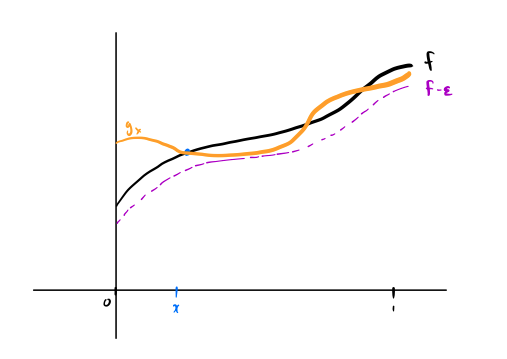
\includegraphics[scale=.5]{weierstrass.png}
	\end{center}
\end{figure}

\begin{proof}
	Take another point $y \in K$, $y \neq x$. By the previous lemma, we can find an $h_y \in \bar{A}$ such that
	\begin{enumerate}
		\item $h_y(x) = f(x)$ 
		\item $h_y(y) = f(y)$
	\end{enumerate}
	Since $h_y$ is continuous, there exists a $\delta_y > 0$ such that
	\begin{equation}
		t \in B_{\delta_y}(y) \imp |h_y(t) - f(t)| < \e
	\end{equation}
	Notice that this implies that $h_y(t) > f(t) - \e$. Now notice that $\parens{B_{\delta_y}(y)}_{y \in K}$ is an open cover of $K$. Compactness implies the existence of a finite subcover, identified by points $y_1, \ldots, y_m$. Now let
	\begin{equation}
		g_x = \max\{h_{y_1},\ldots,h_{y_m}\}
	\end{equation}
	We have, by a previous lemma, that $g_x \in \bar{A}$. Further, it is clear that
	\begin{equation}
		g_x(x) = f(x) 
	\end{equation}
	since each $h_{y_i}(x) = x$ and
	\begin{equation}
		g_x(t) > f(t) - \e
	\end{equation}
	since by taking the max (pointwise) of elements for which this is true. This proves the claim. 
\end{proof}
	\textbf{Finally ready to complete the whole proof.}
\begin{proof}[Proof of Stone-Weierstrass Theorem]
	
\end{proof}













\newpage
\section{Linear Operators and Derivatives}

\section[Differential Calculus in Rn]{Differential Calculus in $\RR^n$}

\section{The Baire category theorem}

\appendix

\section{Review From Elementary Analysis}

\subsection{The Real and Complex Number System}

\begin{definition}[Supremum, Infimum]
	Let $S$ be an ordered set, $E \subset S$, and $E$ be bounded above. Suppose there exists an $\alpha \in S$ with the following properties:
	\begin{enumerate}
		\item $\alpha$ is an upper bound of $E$.
		\item $If \gamma < \alpha$ then $\gamma$ is not an upper bound of $E$.
	\end{enumerate}
	Then $\alpha$ is called the least upper bound of $E$ or \navy{supremum} of $E$ and we write $\alpha = \sup E$. Similarly, $\alpha$ is the greatest lower bound of $E$ or \navy{infimum} of $E$ if 
	\begin{enumerate}
		\item $\alpha$ is a lower bound of $E$.
		\item $If \beta > \alpha$ then $\beta$ is not a lower bound of $E$.
	\end{enumerate}
	and we write $\alpha = \inf E$.
\end{definition}

\begin{definition}[Limit Superior, Inferior]
	Let $\parens{x_n}$ be a sequence of real numbers.

	\begin{enumerate}
		\item The \navy{limit superior} of the sequence is defined by
			\begin{equation}
				\limsup\limits_{n \to \infty} x_n = \lim_{n \to \infty}\parens{\sup_{m \geq n} x_m}
			\end{equation}
			or
			\begin{equation}
				\limsup\limits_{n \to \infty} x_n = \inf_{n \geq 0} \parens{\sup_{m \geq n} x_m} = \inf\Set{\sup \Set{x_m; m \geq n}; n \geq 0}
			\end{equation}

			\textbf{Alternatively}, the limit superior of the sequence is the smallest $b \in \RR$ such that $\forall \e > 0$ $\exists N$ such that $x_n < b + \e$ $\forall n > N$. Thus, any number larger than the limit superior is an upper bound for the sequence after a finite number of terms (hence, only a finite number of elements are greater that $b + \e$).

			\textbf{Alternatively}, the limit superior of the sequence is the supremum of the set of subsequential limits. 

		\item The \navy{limit inferior} of the sequence is defined by
			\begin{equation}
				\liminf\limits_{n \to \infty} x_n = \lim_{n \to \infty}\parens{\inf_{m \geq n} x_m}
			\end{equation}
			or
			\begin{equation}
				\liminf\limits_{n \to \infty} x_n = \sup_{n \geq 0} \parens{\inf_{m \geq n} x_m} = \sup\Set{\inf \Set{x_m; m \geq n}; n \geq 0}
			\end{equation}	
	\end{enumerate}

\end{definition}

\begin{theorem}[Properties of limit superiors]
	Let $\parens{x_n}$ and $\parens{y_n}$ be sequence of real numbers. Then
	\begin{enumerate}
		\item $\limsup\limits_{n \to \infty}(x_n + y_n) \leq \limsup\limits_{n \to \infty} x_n + \limsup\limits_{n \to \infty} y_n$ (as long as the RHS is not of the form $\infty - \infty$)
	\end{enumerate}
\end{theorem}
\begin{proof}
	We prove each item in turn.
	\begin{enumerate}
		\item We have that
		\begin{equation}
			\limsup\limits_{n \to \infty}(x_n + y_n) = \lim_{n \to \infty}\parens{\sup_{m \geq n}\Set{x_m + y_m, x_{m+1} + y_{m+1}, \ldots}}
		\end{equation}
		Then 
		\begin{equation}
			M_n := \sup_{m \geq n}\Set{x_m + y_m, x_{m+1} + y_{m+1}, \ldots} = \sup_{m \geq n}\Set{x_m + y_m} \leq \sup_{m \geq n}\Set{x_m} + \sup_{m \geq n}\Set{y_m}
		\end{equation}
		Take the limit of both sides to get
		\begin{equation}
			\lim_{n \to \infty} M_n \leq \lim_{n \to \infty} \sup_{m \geq n} \Set{x_m} + \lim_{n \to \infty} \sup_{m \geq n} \Set{y_m}
		\end{equation}
		Thus 
		\begin{equation}
			\limsup\limits_{n \to \infty}(x_n + y_n) \leq \limsup\limits_{n \to \infty} x_n + \limsup\limits_{n \to \infty} y_n
		\end{equation}
	\end{enumerate}
\end{proof}



\subsection{Basic Topology}

In what follows, assume $X$ is a metric space. 

\begin{definition}[Limit point]
	A point $p$ is a \navy{limit point} of the set $E$ if every neighborhood of $p$ contains a point $q \neq p$ such that $q \in E$.
\end{definition}

\begin{definition}[Closed]
	$E$ is \navy{closed} if every limit point of $E$ is a point of $E$.
\end{definition}

\begin{definition}[Interior]
	A point $p$ is an \navy{interior point} of $E$ if there is a neighborhood $N$ of $p$ such that $N \subset E$.
\end{definition}

\begin{definition}[Open]
	$E$ is \navy{open} if every point of $E$ is an interior point of $E$.
\end{definition}

\begin{definition}[Bounded]
	$E$ is \navy{bounded} if there is a real number $M$ and a point $q \in X$ such that $d(p,q) < M$ for all $p \in E$.
\end{definition}

\begin{definition}[Separated, Connected]
	Two subsets $A$ and $B$ of a metric space $X$ are said to be \navy{separated} if both $A \cap \bar{B}$ and $\bar{A} \cap B$ are empty (i.e., if no point of $A$ lies in the closure of $B$ and no point of $B$ lies in the closure of $A$). A set $E \subset X$ is said to be \navy{connected} if $E$ is not a union of two nonempty separated sets. 
\end{definition}

\subsection{Numerical Sequences and Series}

\subsubsection{Sequences}

\begin{definition}[Convergent Sequence]
	A sequence $(p_n)$ in a metric space $X$ is said to \navy{converge} if there is a point $p \in X$ such that for every $\e > 0$ there is an integer $N$ such that $n \geq N$ implies $d(p_n,p) < \e$. 
\end{definition}

\begin{definition}[Subsequence, Subsequential Limit]
	Given a sequence $(p_n)$, consider a sequence $(n_k)$ of positive integers such that $n_1 < n_2 < n_3 < \cdots $. Then the sequence $(p_{n_i})$ is called a \navy{subsequence} of $(p_n)$. If $(p_{n_i})$ converges, its limit is called a \navy{subsequential limit} of $(p_n)$.
\end{definition}

Observations:
\begin{itemize}
	\item $(p_n)$ converges to $p$ if and only if every subsequence of $(p_n)$ converges to $p$. 
\end{itemize}

\begin{theorem}[Sequences in compact metric spaces have a convergent subsequence]
	If $(p_n)$ is a sequence in a compact metric space $X$, then some subsequence of $(p_n)$ converges to a point of $X$.
\end{theorem}

\begin{theorem}[Bolzano-Weierstrass]
	Every bounded sequence in $\RR^k$ has a convergent subsequence.
\end{theorem}

\begin{definition}[Cauchy Sequence]
	A sequence $(p_n)$ in a metric space $X$ is said to be a \navy{Cauchy Sequence} if for every $\e > 0$ there is an integer $N$ such that $d(p_n, p_m) < \e$ if $n \geq N$ and $m \geq N$.
\end{definition}

\begin{definition}[Diameter]
	Let $E$ be a nonempty subset of a metric space $X$, and let $S$ be the set of all real numbers of the form $d(p,q)$ with $p \in E$ and $q \in E$. The sup of $S$ is called the \navy{diameter} of $E$.
\end{definition}

\begin{theorem}[Facts about Cauchy sequences]
	We have that
\begin{enumerate}
	\item In any metric space $X$, every convergent sequence is a Cauchy sequence.
	\item If $X$ is a compact metric space and if $(p_n)$ is a Cauchy sequence in $X$, then $(p_n)$ converges to some point of $X$.
	\item In $\RR^k$, every Cauchy sequence converges. 
\end{enumerate}
\end{theorem}

\begin{definition}[Complete]
	A metric space in which every Cauchy sequence converges is \navy{complete}.
\end{definition}

\begin{definition}[Monotonically increasing, decreasing]
	A sequence $(s_n)$ of real numbers is said to be
	\begin{enumerate}
		\item \navy{Monotonically increasing} if $s_n \leq s_{n_1}$ for all $n$.
		\item \navy{Monotonically decreasing} if $s_n \geq s_{n_1}$ for all $n$.
	\end{enumerate}
\end{definition}

\begin{theorem}[Convergence of monotonic sequences]
	Let $(s_n)$ be a monotonic sequence. Then $(s_n)$ converges if and only if it is bounded. 
\end{theorem}

\subsubsection{Series}

\begin{definition}[Convergent Series]
	Let $\sum_{n=1}^\infty a_n$ be an infinite series. Define $s_n = \sum_{k=1}^n a_n$ to be the $n$th partial sum of the series. If the sequence of partial sums $\Set{s_n}$ converges to $s$, we say the series $\navy{converges}$.  
\end{definition}

\begin{theorem}[Cauchy Criterion for Series]
	$\sum a_n$ converges iff
	\begin{equation}
		\forall \e > 0 \ \exists N \text{ s.t. } m,n \geq N \imp \abs{\sum_{k=n}^m a_k} \leq \e
	\end{equation}
\end{theorem}

\begin{theorem}[Necessary condition for convergence: individual terms of series go to $0$.]
	If $\sum a_n$ converges, then $\lim_{n \to \infty} a_n = 0$. 
\end{theorem}

\begin{theorem}[]
	A series of nonnegative terms converges if and only if its partial sums form a bounded sequence. 
\end{theorem}

\begin{theorem}[Root Test]
	Given $\sum a_n$, let $\alpha = \limsup\limits_{n \to \infty} \sqrt[n]{\abs{a_n}}$. Then
	\begin{enumerate}
		\item If $\alpha < 1$, $\sum a_n$ converges.
		\item If $\alpha > 1$, $\sum a_n$ diverges.
		\item If $\alpha = 1$, the test gives no information. 
	\end{enumerate}
\end{theorem}




\subsection{Continuity}

\begin{definition}[Limit]
	Let $X$ and $Y$ be metric spaces, $E \subset X$, $f$ map $E$ into $Y$, and $p$ be a limit point of $E$. We write $f(x) \to q$ as $x \to p$ or $\navy{\lim_{x\to p} f(x) = q}$ if there is a point $q \in Y$ such that for every $\e > 0$ there exists a $\d > 0$ such that for all $x \in E$ for which $0 < d_X(x,p) < \d$, we have $d_Y(f(x),q) < \e$. 
\end{definition}

\begin{definition}[Continuous]
	Suppose $X$ and $Y$ are metric spaces, $E \subset X$, $p \in E$, and $f$ maps $E$ into $Y$. Then $f$ is \navy{continuous} at $p$ if for every $\e > 0$ there there exists a $\d > 0$ such that for all $x \in E$ for which $d_X(x,p) < \d$, we have that $d_Y(f(x), f(p)) < \e$. 
\end{definition}

\begin{definition}[Uniformly Continuous]
	Let $f$ be a mapping of a metric space $X$ into a metric space $Y$. We say that $f$ is \navy{uniformly continuous} on $X$ if for every $\e > 0$ there exists a $\d > 0$ such that for all $p,q \in X$ for which $d_X(p,q) < \delta$, we have $d_Y(f(p),f(q)) < \e$. 
\end{definition}

Observations:
\begin{itemize}
	\item Uniform continuity is a property of a function on a set, whereas continuity can be defined at a single point. 
	\item If $f$ is continuous on $X$, then for each $\e > 0$ and each $p \in X$, we can find a $\d > 0$ that satisfies the condition in the definition. For uniform continuity, we can find one $\d > 0$ that works for all points $p \in X$. 
	\item Every uniformly continuous function is continuous. The two concepts are equivalent on compact sets. 
\end{itemize}

\subsection{Differentiation}

\begin{definition}[Differentiable, Derivative]
	Let $f$ be defined (and real-valued) on $[a,b]$. For any $x \in [a,b]$ define
	\begin{equation}
		f'(x) = \lim_{t \to x} \frac{f(t) - f(x)}{t - x}
	\end{equation}
	provided this limit exists. If $f'$ is defined at a point $x$, we say that $f$ is \navy{differentiable} at $x$. $f'$ is called the \navy{derivative} of $f$.  
\end{definition}

\begin{theorem}[Mean Value Theorem]
	If $f$ is a real continuous function on $[a,b]$ which is differentiable on $(a,b)$, then there is a point $x \in (a,b)$ at which 
	\begin{equation}
		f(b) - f(a) = (b - a) f'(x)
	\end{equation}
\end{theorem}

% \section{Functions of Several Variables}

% \subsection{Differentiation}

% \begin{definition}[Differentiable]
% 	Let $V,W$ be normed vector spaces. Let $U \subset V$ be an open subset of $V$ and let $f: U \to W$ be a function. Fix $a \in U$. $f$ is \navy{differentiable} at $a$ if there exists a bounded linear transformation $T: V \to W$ (denoted $Df_a or f'(a)$) such that
% 	\begin{equation}
% 		\lim_{h\to 0} \frac{\norm{f(a+h) - f(a) - Th}_W}{\norm{h}_V} = 0
% 	\end{equation}
% \end{definition}


% \subsection{Contraction Principle}

% \begin{definition}[Contraction]
% 	Let $X$ be a metric space, with metric $d$. If $\phi$ maps $X$ into $X$ and if there is a number $c < 1$ such that
% 	\begin{equation}
% 		d(\phi(x),\phi(y)) \leq c d(x,y)
% 	\end{equation}
% 	for all $x,y \in X$, then $\phi$ is a \navy{contraction} of $X$ into $X$.
% \end{definition}

% Observations:
% \begin{itemize}
% 	\item Contractions are continuous: Let $x \in X$ and fix $\e > 0$. Set $\d = \frac{\e}{c}$. Then for all $y \in X$ such that $d(x,y) < \d$, we have that
% 	\begin{equation*}
% 		d(\p(x), \p(y)) \leq c d(x,y) \leq c \cdot \frac{\e}{c} = \e
% 	\end{equation*}
% \end{itemize}

% \begin{theorem}[Banach Fixed-Point Theorem]
% 	If $X$ is a complete metric space, and if $\p$ is a contraction of $X$ into $X$, then there exists a unique $x \in X$ such that $\p(x) = x$.
% \end{theorem}
% \begin{proof}
% 	We first prove uniqueness, then existence. 

% 	\textbf{Uniqueness:} Suppose $x,y \in X$ are fixed points of $\p$. Then
% 	\begin{align*}
% 		0 &\leq d(x,y) \tag{distances positive} \\
% 		&= d(\p(x), \p(y)) \tag{$x,y$ fixed points} \\
% 		&\leq c \cdot d(x,y) \tag{$\p$ a contraction}	
% 	\end{align*}
% 	Since $c \in (0,1)$, we must have that $d(x,y) = 0$. Therefore $x=y$. 

% 	\textbf{Existence:} Fix an $x_0 \in X$ and define a sequence $(x_n)_n$ by
% 	\begin{equation}
% 		x_{n+1} = \p(x_n)
% 	\end{equation}
% 	We now show $(x_n)_n$ is a Cauchy sequence. Observe that
% 	\begin{equation*}
% 		d(x_{n+1},x_n) = d(\p(x_n), \p(x_{n-1})) \leq c d(x_n, x_{n-1}) \leq c^2 d(x_{n-1}, x_{n-2}) \leq \cdots \leq c^n d(x_1, x_0)
% 	\end{equation*}
% 	Fix an arbitrary $m,n \in \ZZ$, $m > n$. Then
% 	\begin{align*}	
% 		d(x_m, x_n) &\leq d(x_m, d_{m-1}) + d(d_{m-1},d_{m-2}) + \cdots + d(x_{n+1}, x_n) \tag{triangle inequality} \\
% 		&= \sum_{i=n}^{m-1} d(x_{i+1}, x_i) \\
% 		&\leq \sum_{i=n}^{m-1} c^i d(x_1, x_0) \tag{contraction} \\
% 		&\leq d(x_1, x_0) \sum_{i=n}^\infty c^i \\
% 		&= c^n \frac{d(x_1, x_0)}{1-c} \tag{geometric series}
% 	\end{align*}
% 	Therefore as $n \to \infty$, since $c \in (0,1)$, $c^n \to 0$. Thus $d(x_m, x_n) \to 0$. Therefore $(x_n)_n$ is a Cauchy sequence. By completeness of $X$, $(x_n)_n$ must converge to a limit in $p \in X$. $\p$ is continuous since it is a contraction. Therefore
% 	\begin{align*}
% 		\p(p) &= \p(\lim_{n\to \infty} x_n) \\
% 		&= \lim_{n\to \infty} \p(x_n) \tag{by continuity} \\
% 		&= \lim_{n\to \infty} x_{n+1} \tag{definition of $\p$} \\
% 		&= p	
% 	\end{align*}
% 	Therefore $p$ is a fixed point.  				 				
% \end{proof}

% \subsection{The Inverse Function Theorem}
% ``A continuously differentiable mapping $f$ is invertible in a neighborhood of any point $x$ at which the linear transformation $f'(x)$ is invertible.''

\newpage
\nocite{*}
\bibliography{references}
\bibliographystyle{apalike}

\end{document}